\begin{figure}[H]
\centering
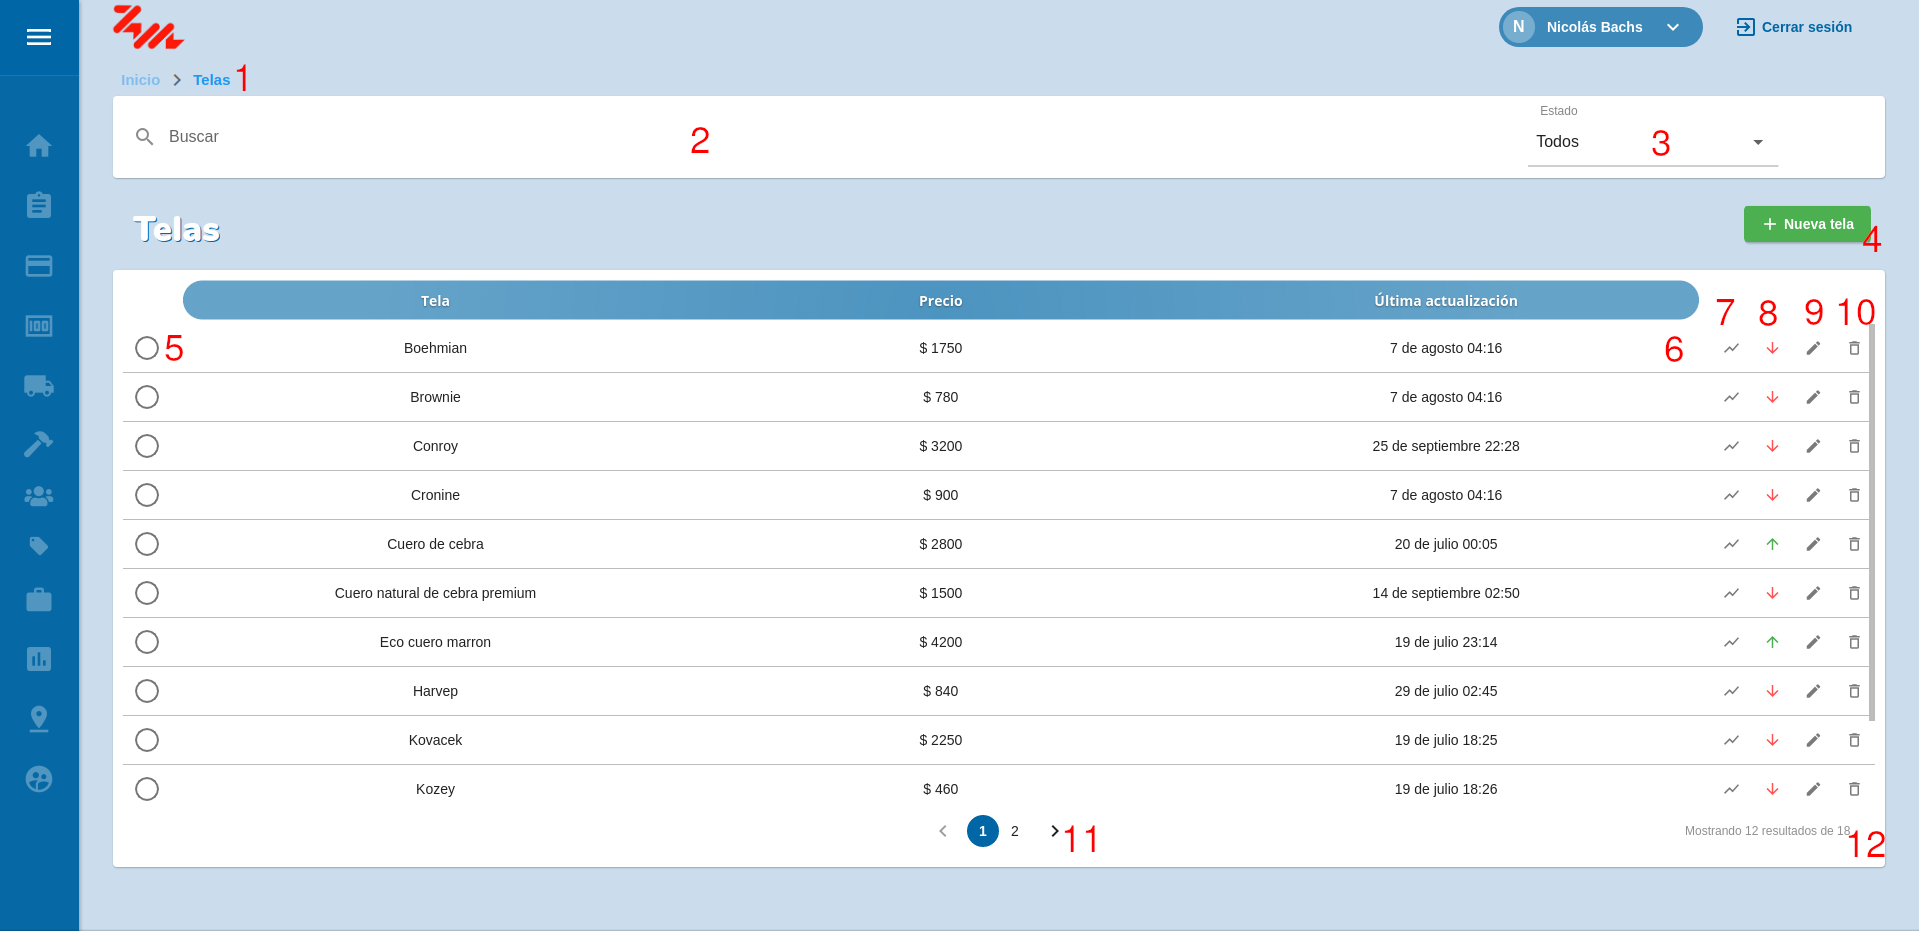
\includegraphics[width=\textwidth,height=\textheight,keepaspectratio]{Escenarios/AD-39-00}
\caption{Escenario - AD-39-00}
\label{fig:AD-39-00}
\end{figure}

Este escenario muestra toda la información referida a las telas, junto con las acciones disponibles.
El botón \textbf{AD-42-01} permite navegar al escenario \textbf{AD-02-00}. El campo \textbf{AD-42-02} permite ingresar un texto para filtrar las telas por nombre y la lista desplegable \textbf{AD-42-03} permite al usuario filtrar por los estados en los cuales puede encontrarse la tela.

El botón \textbf{AD-42-04} permite al usuario crear una nueva tela y navega al escenario \textbf{AD-40-00}.
El botón \textbf{AD-42-05} permite al usuario seleccionar una o más telas del resultado de la búsqueda. Si existen telas seleccionadas se mostrarán botones con las opción de borrar o activar/desactivar según corresponda. El campo \textbf{AD-42-06} muestra la información relacionada a las telas especificando el código, nombre de la tela, precio actual y cuándo se realizó la última actualización del precio. El botón \textbf{AD-42-07} permite navegar al escenario \textbf{AD-41-00} para ver los precios de la tela, el botón \textbf{AD-42-08} permite al usuario dar de alta/baja una tela, el botón \textbf{AD-42-09} permite al usuario editar la tela navegando al escenario \textbf{AD-40-00} y el botón \textbf{AD-42-10} permite al usuario borrar la tela. 
En \textbf{AD-42-11} se mostrarán las páginas de resultado, pudiendo cambiar de página. En \textbf{AD-42-12} se mostrará cuantos resultados se están visualizando y el total.
\clearpage
